\def\difficulty{1}
\sujet{Introduction to image processing}


\begin{note}
In this tutorial, you will discover the basic functions in order to load, manipulate and  display images. The main informations of the images will be retrieved, like size, number of channels, storage class, etc. Afterwards, you will be able to perform your first classic filters.
\end{note}

\noindent The different processes will be realized on the following images:

\vspace*{-8pt}
\begin{figure}[htbp]
\centering\caption{Image examples.}
\subfloat[Retinal vessels.]{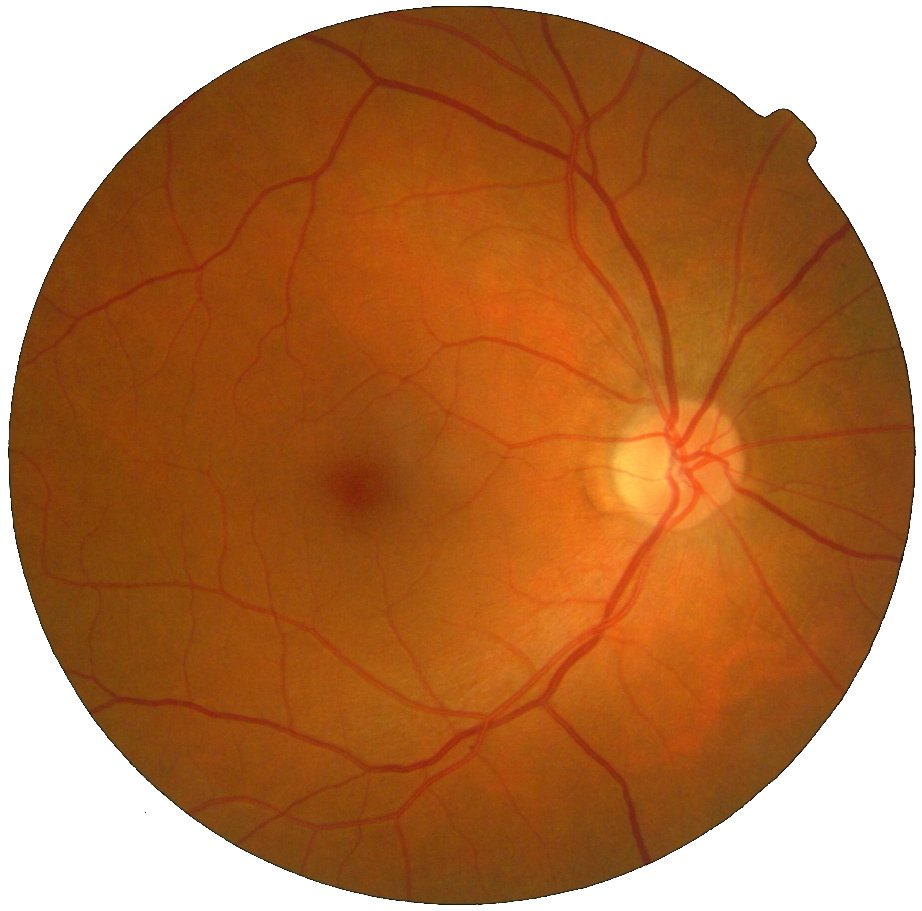
\includegraphics[height=.28\linewidth]{retine.png}}
\hfill
\subfloat[Muscle cells.]{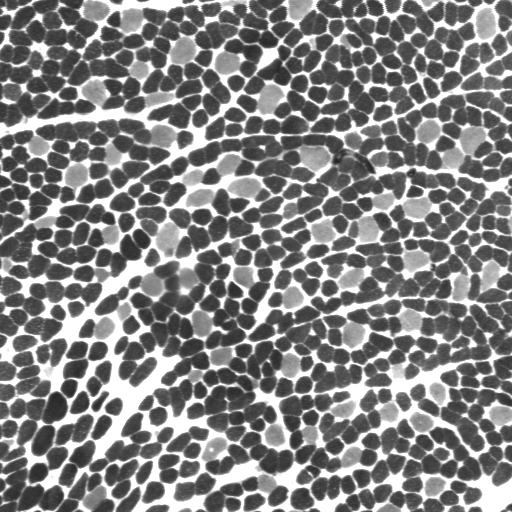
\includegraphics[height=.3\linewidth]{muscle.jpg}}
\hfill
\subfloat[Cornea cells (BIIGC, Univ. Jean Monnet, Saint-Etienne, France).]{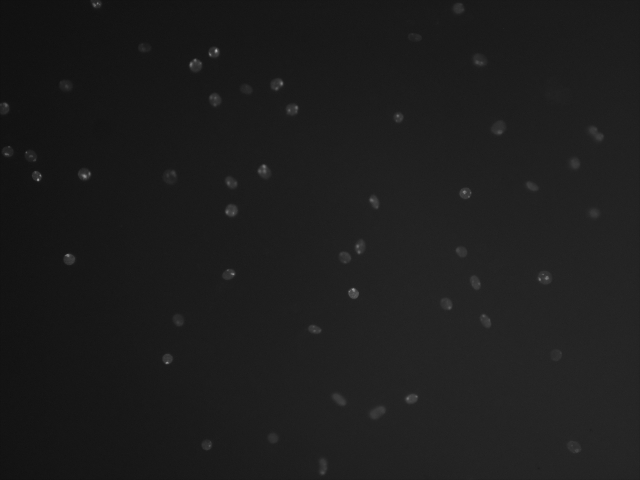
\includegraphics[height=.3\linewidth]{cellules_cornee.jpg}}
\vspace*{-10pt}
\end{figure}

\vspace*{-15pt}

%%%%%%%%%%%%%%%%%%%%%%%%%%%%%%%%%%%%%%%%%%%%%%%%%%%%%%%%%%%%%%%%%%%%%%%%%%%%%%%%%%%%%%%%

\section{First manipulations}
\index{Image!Load}\index{Image!Display}

\begin{pcomment}
\begin{premark}Image loading can be made by the use of the python function \pinline{imageio.imread}.
The visualization of the image in the screen is realized by using the module \pinline{matplotlib.pyplot}.
\end{premark}
\end{pcomment}

\begin{mcomment}
\begin{mremark}Image loading can be made by the use of the \matlabregistered{} function \minline{imread}. 
The visualization of the image in the screen is realized either by the \matlabregistered{} function \minline{imagesc} or \minline{imshow}.
\end{mremark}
\end{mcomment}

\begin{qbox}
\begin{itemize}
\item Load and visualize the first image as below. Notice the differences.
 \item Look at the data structure of the image $I$ such as its size, type\dots.
\item Visualize the green component of the image.
Is it different from the red one? What is the most contrasted color component? Why? 
\item Enumerate some digital image file formats. 
What are their main differences? 
Try to write images with the JPEG file format with different compression ratios (0, 50 and 100), as while as the lossless compression, and compare.
\end{itemize}
\end{qbox}

\begin{mcomment}
 \begin{mremark}
  See \minline{imwrite}.
 \end{mremark}
\end{mcomment}

%%%%%%%%%%%%%%%%%%%%%%%%%%%%%%%%%%%%%%%%%%%%%%%%%%%%%%%%%%%%%%%%%%%%%%%%%%%%%%%%%%%%%%%%%%%%%%%%%%%
\section{Color quantization}
\index{Quantization}
Color quantization is a process that reduces the number of distinct colors used in an image, usually with the intention that the resulting image should be as visually similar as possible to the original image. In principle, a color image is usually quantized with 8 bits (i.e. 256 gray levels) for each color component.

\begin{qbox}
\begin{itemize}
\item By using the gray level image 'muscle', reduce the number of gray levels to  128, 64, 32, and visualize the different resulting images.
\item Compute the different image histograms and compare. 
\end{itemize}
\end{qbox}



%%%%%%%%%%%%%%%%%%%%%%%%%%%%%%%%%%%%%%%%%%%%%%%%%%%%%%%%%%%%%%%%%%%%%%%%%%%%%%%%%%%%%%%%%%%%%%%%%%%
\vspace*{-8pt}
\section{Image histogram}
\index{Histogram}
An image histogram represents the gray level distribution in a digital image.
The histogram corresponds to the number of pixels for each gray level.
\begin{mcomment}
The \matlabregistered{} function that computes the histogram of any gray level image has the following prototype:
\begin{matlab}
function h = histogram(I)
\end{matlab}
\end{mcomment}

\begin{pcomment}
The python function has the following prototype:
\begin{python}
def histogram(I):
\end{python}
\end{pcomment}

\begin{qbox}
Compute and visualize the histogram of the image 'muscle.jpg'.
\end{qbox}


%%%%%%%%%%%%%%%%%%%%%%%%%%%%%%%%%%%%%%%%%%%%%%%%%%%%%%%%%%%%%%%%%%%%%%%%%%%%%%%%

\vspace*{-8pt}
\section{Linear mapping of the image in\-ten\-si\-ties}

The gray level range of the image 'cellules\_cornee.jpg' can be enhanced by a linear map\-ping such that the minimum (resp. maximum) gray level value of the resulting image is $0$ (resp. $255$). Mathematical\-ly, it consists in finding a function $f(x)=ax+b$ such that 
$f(min)=0$ and $f(max)=255$.

\begin{qbox}
\begin{itemize}
\item Load the image and find its extremal gray level values.
\item Adjust the intensities by a linear mapping into $[0, 255]$.

\item Visualize the resulting image and its histogram.
\end{itemize}
\end{qbox}

\vspace*{-8pt}

\section{Aliasing effect}
\index{Aliasing}

\begin{qbox}
	\begin{minipage}{0.6\textwidth}
\begin{itemize}
\item Create an image (as right) that contains rings as sinusoids. The function takes two input parameters: the sampling frequency and the signal frequency.
%\begin{center}
%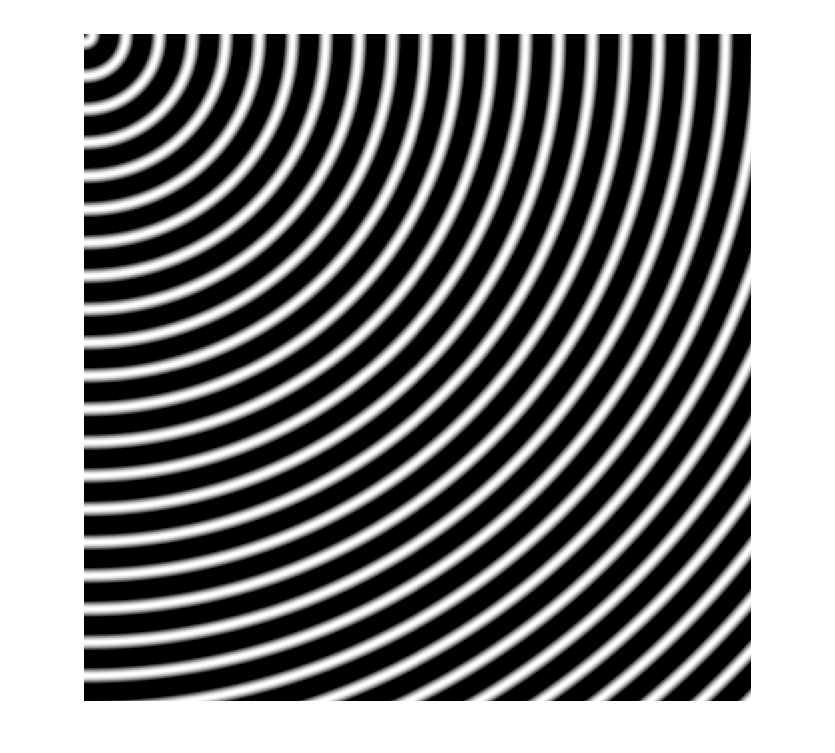
\includegraphics[height=3.5cm]{moire.png}
%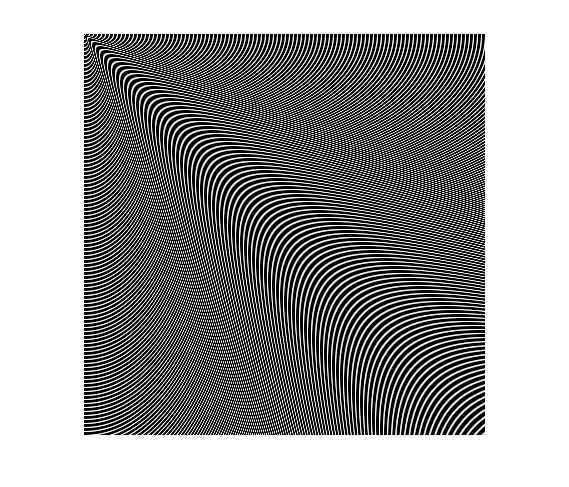
\includegraphics[height=4.25cm]{moire2.png}
%\end{center}
\item Look at the influence of the two varying frequencies. What do you observe? Explain the phenomenon from a theoretical point of view.
\end{itemize}
\end{minipage}
\hfill
\begin{minipage}{0.35\textwidth}
	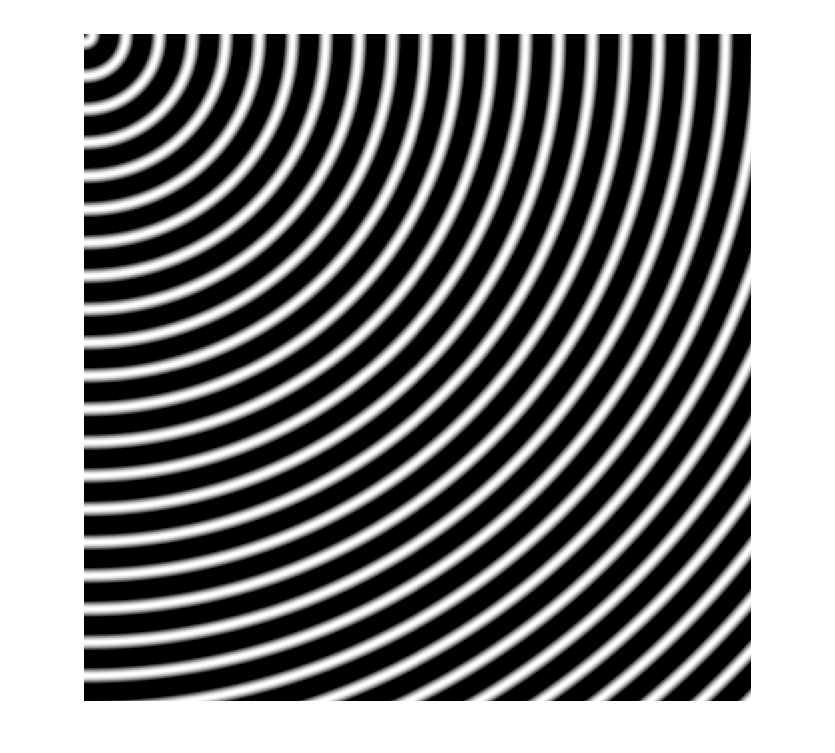
\includegraphics[height=3.5cm]{moire.png}
\end{minipage}
\end{qbox}

%%%%%%%%%%%%%%%%%
% filtering


\section{Low-pass filtering}
\index{Filtering!Low-pass}\index{Filtering!Convolution}

The different processes will be realized on the following images:
{
	\makeatletter
	\renewcommand\fs@ruled{\def\@fs@cfont{\bfseries}\let\@fs@capt\floatc@ruled
		\def\@fs@pre{\hrule height.8pt depth0pt \kern2pt}%
		\def\@fs@post{\kern2pt\hrule\relax}%
		\def\@fs@mid{\vskip2pt}%
		\let\@fs@iftopcapt\iftrue}
	\makeatother
\begin{figure}[H]
\centering
\subfloat[osteoblast cells]{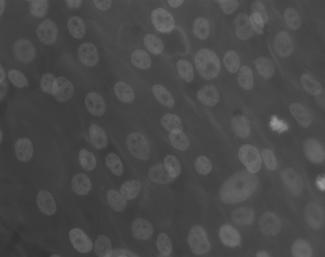
\includegraphics[height=4.5cm]{osteoblaste.jpg}}
\hfill
\subfloat[blood cells]{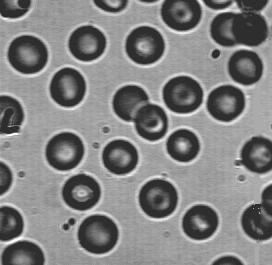
\includegraphics[height=4.5cm]{blood.jpg}}
\vspace*{-10pt}
\end{figure}
}

Low-pass filtering aims to smooth the fast intensity variations of the image to be processed.
\begin{qbox}
Test the low-pass filters 'mean', 'median', 'min', 'max' and 'gaussian' on the noisy image 'blood cells'. 
\end{qbox}

	\begin{mcomment}
\begin{mremark}The \matlabregistered{} functions \minline{imfilter} and \minline{nlfilter} can be employed.
Be careful to the function options for border problems. Also, the \matlabregistered{} function \minline{fspecial} enables an operational window to be generated.
\end{mremark}
\end{mcomment}

\begin{pcomment}
\begin{premark}
The module \pinline{scipy.ndimage.filters} contains a lot of classical filters.
\end{premark}
\end{pcomment}
\begin{qbox}
Which filter is suitable for the restoration of this image?
\end{qbox}

%%%%%%%%%%%%%%%%%%%%%%%%%%%%%%%%%%%%%%%%%%%%%%%%%%%%%%%%%%%%%%%%%%%%%%%%%%%%%%%%%%%%%%%%%%%%%%%%%%%
\section{High-pass filtering}
\index{Filtering!High-pass}
\index{Laplacian}

High-pass filtering aims to smooth the low intensity variations of the image to be processed.
\begin{qbox}
\begin{itemize}
	\item Test the high-pass filters $HP$ on the two initial images in the following way: 
	$HP(f)=f-LP(f)$ where $LP$ is a low-pass filtering (see the previous exercise).
	\item Test the Laplacian \label{lbl:introduction:laplacien}(high-pass) filter on the two initial images with the following convolution mask:
$$
\left[
\begin{array}{ccc}
-1&-1&-1\\
-1&+8&-1\\
-1&-1&-1
\end{array}
\right]
$$
\end{itemize}
\end{qbox}


\section{Derivative filters}
\index{Gradient!Prewitt}
\index{Gradient!Sobel}

Derivative filtering aims to detect the edges (contours) of the image to be processed.
\begin{qbox}
\begin{itemize}
	\item
Test the Prewitt and Sobel derivative filters (corresponding to first order derivatives) on the image 'blood cells' with the use of the following convolution masks:
$$
\left[
\begin{array}{ccc}
-1&0&+1\\
-1&0&+1\\
-1&0&+1
\end{array}
\right]
\left[
\begin{array}{rrr}
-1&-1&-1\\
0&0&0\\
+1&+1&+1
\end{array}
\right]
$$
$$
\left[
\begin{array}{ccc}
-1&0&+1\\
-2&0&+2\\
-1&0&+1
\end{array}
\right]
\left[
\begin{array}{rrr}
-1&-2&-1\\
0&0&0\\
+1&+2&+1
\end{array}
\right]
$$
\item Look at the results for the different gradient directions.
\item Define an operator taking into account the horizontal and vertical directions.
\end{itemize}
\end{qbox}

Remark : the edges could be also detected with the zero-cressings of the Laplacian filtering  (corresponding to second order derivatives).

 

\section{Enhancement filtering}
Enhancement filtering aims to enhance the contrast or accentuate some specific image characteristics.
\begin{qbox}
\begin{itemize}
	\item Test the enhancement filter $E$ on the image 'osteoblast cells' defined as:
	$E(f)=f+HP(f)$ where $HP$ is a Laplacian filter (see  \iflabelexists{tutorial:image_enhancement}{tutorial \ref{tutorial:image_enhancement}.}{tutorial about enhancement.}).
	\item Parameterize the previous filter as:
	$E(f)=\alpha f+HP(f)$, where $\alpha\in\mathbb{R}$.
\end{itemize}
\end{qbox}

\section{Open question}
Find an image filter for enhancing the gray level range of the image 'osteoblast cells'.

